\documentclass[12pt,]{article}
\usepackage{lmodern}
\usepackage{amssymb,amsmath}
\usepackage{ifxetex,ifluatex}
\usepackage{fixltx2e} % provides \textsubscript
\ifnum 0\ifxetex 1\fi\ifluatex 1\fi=0 % if pdftex
  \usepackage[T1]{fontenc}
  \usepackage[utf8]{inputenc}
\else % if luatex or xelatex
  \ifxetex
    \usepackage{mathspec}
  \else
    \usepackage{fontspec}
  \fi
  \defaultfontfeatures{Ligatures=TeX,Scale=MatchLowercase}
\fi
% use upquote if available, for straight quotes in verbatim environments
\IfFileExists{upquote.sty}{\usepackage{upquote}}{}
% use microtype if available
\IfFileExists{microtype.sty}{%
\usepackage{microtype}
\UseMicrotypeSet[protrusion]{basicmath} % disable protrusion for tt fonts
}{}
\usepackage[margin=1in]{geometry}
\usepackage{hyperref}
\hypersetup{unicode=true,
            pdftitle={Fiche descriptive du script R},
            pdfauthor={Jules Corbel},
            pdfborder={0 0 0},
            breaklinks=true}
\urlstyle{same}  % don't use monospace font for urls
\usepackage{graphicx,grffile}
\makeatletter
\def\maxwidth{\ifdim\Gin@nat@width>\linewidth\linewidth\else\Gin@nat@width\fi}
\def\maxheight{\ifdim\Gin@nat@height>\textheight\textheight\else\Gin@nat@height\fi}
\makeatother
% Scale images if necessary, so that they will not overflow the page
% margins by default, and it is still possible to overwrite the defaults
% using explicit options in \includegraphics[width, height, ...]{}
\setkeys{Gin}{width=\maxwidth,height=\maxheight,keepaspectratio}
\IfFileExists{parskip.sty}{%
\usepackage{parskip}
}{% else
\setlength{\parindent}{0pt}
\setlength{\parskip}{6pt plus 2pt minus 1pt}
}
\setlength{\emergencystretch}{3em}  % prevent overfull lines
\providecommand{\tightlist}{%
  \setlength{\itemsep}{0pt}\setlength{\parskip}{0pt}}
\setcounter{secnumdepth}{5}
% Redefines (sub)paragraphs to behave more like sections
\ifx\paragraph\undefined\else
\let\oldparagraph\paragraph
\renewcommand{\paragraph}[1]{\oldparagraph{#1}\mbox{}}
\fi
\ifx\subparagraph\undefined\else
\let\oldsubparagraph\subparagraph
\renewcommand{\subparagraph}[1]{\oldsubparagraph{#1}\mbox{}}
\fi

%%% Use protect on footnotes to avoid problems with footnotes in titles
\let\rmarkdownfootnote\footnote%
\def\footnote{\protect\rmarkdownfootnote}

%%% Change title format to be more compact
\usepackage{titling}

% Create subtitle command for use in maketitle
\newcommand{\subtitle}[1]{
  \posttitle{
    \begin{center}\large#1\end{center}
    }
}

\setlength{\droptitle}{-2em}
  \title{Fiche descriptive du script R}
  \pretitle{\vspace{\droptitle}\centering\huge}
  \posttitle{\par}
  \author{Jules Corbel}
  \preauthor{\centering\large\emph}
  \postauthor{\par}
  \predate{\centering\large\emph}
  \postdate{\par}
  \date{25/02/2019}

\usepackage{inputenc}

\begin{document}
\maketitle

{
\setcounter{tocdepth}{2}
\tableofcontents
\clearpage
}
\section*{Introduction}\label{introduction}
\addcontentsline{toc}{section}{Introduction}

Cette fiche a pour but de présenter le code écrit dans le cadre du
projet ``Identification de modèles de séries temporelles pour la
prévision de la masse salariale en fonction d'informations auxiliaires''
réalisé en 2018 par Jules Corbel et Paul Guillotte sous la tutelle de M.
Assi N'Guessan. Pour plus de précisions par rapport à des notations,
merci de vous référer à notre rapport sur ce projet (Corbel and
Guillotte 2019).

Le script se décompose en deux parties : un script \textbf{fonctions.R}
contenant toutes les fonctions que nous avons créées afin d'automatiser
des traitements et un script \textbf{main.R} pour tout les traitements.

Les différentes phases du traitement sont résumées par le schéma
ci-dessous.

\begin{figure}[htbp]
\centering
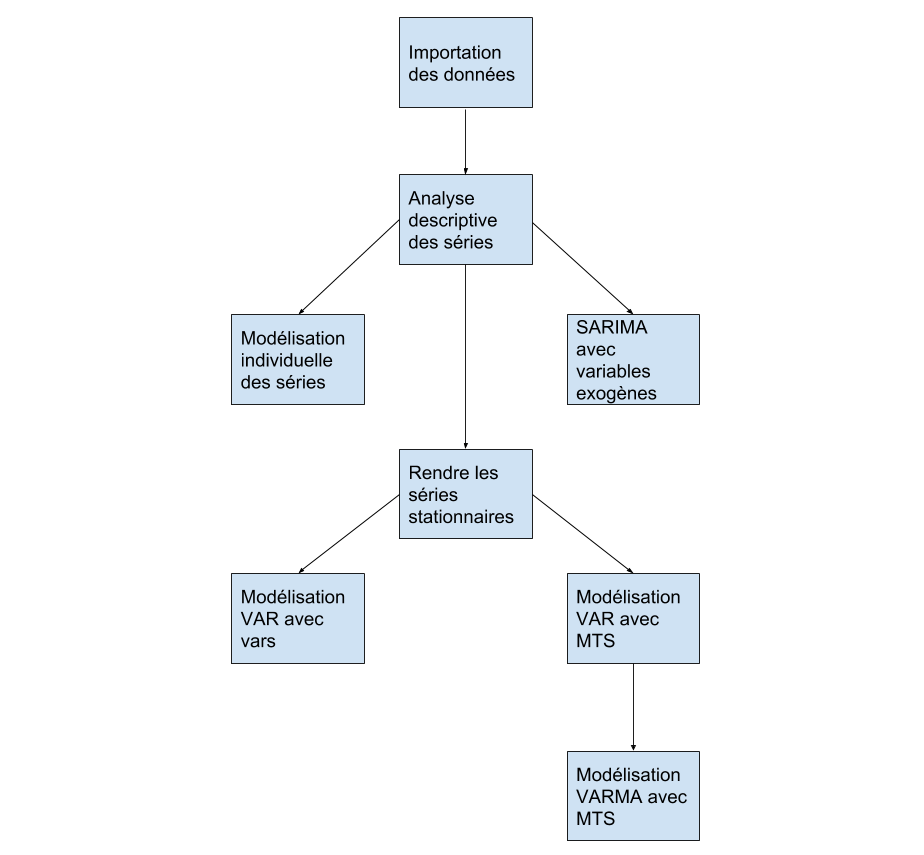
\includegraphics{figures/Schema_script.png}
\caption{Etapes du projet}
\end{figure}

\section{Importation des packages}\label{importation-des-packages}

Afin de réaliser notre projet nous avons eu besoin d'installer un
certain nombre de packages R. La liste est la suivante :

\begin{itemize}
\tightlist
\item
  \textbf{tseries} qui contient le test de racines unitaires
  \emph{adf.test}.
\item
  \textbf{forecast} permettant d'effectuer des prévisions sur les
  modèles (lissage exponentiel, modèlesARMA, modèles VAR avec le package
  \textbf{vars}). L'utilisation de ce package est décrite dans un
  article de Rob J. Hyndman (Hyndman and Khandakar 2008)
\item
  \textbf{corrplot} pour obtenir des visualisations plus parlantes de la
  matrice des corrélations
\item
  \textbf{vars} qui nous permet de réaliser des modèles VAR. La vignette
  de ce package, écrite par Bernhard Pfaff (Pfaff 2018), résume
  parfaitement le contenu de ce package et comment l'utiliser.
\end{itemize}

Nous utilisons également le package \textbf{MTS} pour construire des
modèles VAR et VARMA, mais il n'est pas importé ici en raison de
conflits avec le package \textbf{vars} sur le nom des fonctions.

\section{Importation des données}\label{importation-des-donnees}

La ligne suivante du script est celle de l'importation du jeu de
données. Il faut changer le chemin de la fonction par celui ou est
stocké le jeu de données de l'IRCEM.

\section{Analyse descriptive des
séries}\label{analyse-descriptive-des-series}

Dans cette partie, nous commençons par transformer chacune des colonnes
de notre jeu de données en série temporelle, allant du premier trimestre
de 1990 au deuxième de 2017. Nous visualisons ensuite chacune des séries
graphiquement, leurs fonctions d'autocorrélation. et testons si elles
sont stationnaires grâce au test de KPSS et au test de Dickey-Fuller
augmenté testant la présence de racines unitaires. Nous terminons par le
découpage des séries en échantillons d'apprentissage et de test.

\section{Modélisation individuelle des
séries}\label{modelisation-individuelle-des-series}

Cette partie se décompose en deux : la réalisation de modèles par
lissage exponentiel puis par processus ARMA sur chacune des séries. Nous
visualisons les résultats grâce à l'AICc et à l'erreur quadratique
moyenne, résultats qui sont comparés à la fin de la partie. Nous
estimons également la valeur du PIB pour le deuxième trimestre de 2017,
puisque nous ne l'avons pas, à l'aide du meilleur des deux modèles pour
cette série.

\section{Modélisation ARMA avec variables
exogènes}\label{modelisation-arma-avec-variables-exogenes}

Comme pour la modélisation individuelle, nous effectuons tous les
modèles possibles, soit en utilisant toutes les combinaisons de
variables auxiliaires. Les résultats sont présentés à la fin dans la
matrice \emph{resultats}.

\section{Stationnarisation des
séries}\label{stationnarisation-des-series}

Cette partie est indispensable pour la construction des modèles VAR. En
effet, chacune des séries est stationnarisée grâce à la fonction
\emph{decompose} permettant de séparer la composante de tendance, la
composante saisonnière et la composante résiduelle dans une série. Nous
conservons donc uniquement la composante résiduelle pour toutes les
séries. Nous vérifions que ces composantes sont bien stationnaires grâce
aux mêmes méthodes que précédemment (fonctions ACF et PACF, test KPSS et
test de Dickey-Fuller augmenté). Nous gardons toutefois les composantes
de tendances et de saisonnalité pour la variable MSE, car elles nous
serviront à reconstruire la série et donc effectuer des prévisions.

\section{Mise en place de modèles VAR avec
vars}\label{mise-en-place-de-modeles-var-avec-vars}

Pour toutes les combinaisons de variables comprenant la MSE, nous
déterminons les ordres du modèles associés à chacun des critères à notre
disposition et estimons un modèle pour chacun de ces ordres. Nous
vérifions ensuite que les hypothèses associées au modèle VAR sont bien
respectéeset calculons l'erreur quadratique moyenne pour chaque modèle
et visualisons graphiquement les prédictions par rapport à la série
réelle. Le tableau à la fin de la partie nous donne l'erreur quadratique
moyenne pour le meilleur modèle en terme de prédiction par combinaison
de variables.

\section{Mise en place de modèles VAR avec
MTS}\label{mise-en-place-de-modeles-var-avec-mts}

La méthodologie adoptée est la même qu'avec le package \textbf{vars}, à
ceci près que ce package contient moins de moyens de vérifier les
hypothèses du modèle, nous n'avons donc vérifié que celles qui étaient
possibles.

\section{Mise en place de modèles VARMA avec
MTS}\label{mise-en-place-de-modeles-varma-avec-mts}

Nous terminons par la construction d'un modèle VARMA. Nous commençons
par estimer l'ordre du modèle grâce au calcul des matrices de
corrélation croisée étendues. Nous construisons ensuite le modèle, dont
un grand nombre de paramètres n'est pas significatif. Nous tentons donc
de supprimer les paramètres non significatifs, mais sans succès.

\newpage

\section*{References}\label{references}
\addcontentsline{toc}{section}{References}

\hypertarget{refs}{}
\hypertarget{ref-rapport}{}
Corbel, Jules, and Paul Guillotte. 2019. \emph{Identification de Modeles
de Series Temporelles Pour La Prevision de La Masse Salariale En
Fonction d'informations Auxiliaires}.

\hypertarget{ref-forecast}{}
Hyndman, J., Rob, and Yeasmin Khandakar. 2008. ``Automatic Time Series
Forecasting: The Forecast Package for R.'' \emph{Journal of Statistic
Software}, July.

\hypertarget{ref-vars}{}
Pfaff, Bernhard. 2018. \emph{VAR, Svar and Svec Models: Implementation
Within R Package Vars}.

\hypertarget{ref-MTS}{}
Tsay, Ruey S., and David Wood. 2002. \emph{Analysis of Financial Time
Series}. Wiley-Science Interproduction.


\end{document}
